\chapter{Game Design} 
	\section{Methodology}
		\par My \textbf{approach} resembled \textbf{Iterative Game Designing} the most. \textbf{Trying new things, testing, discarding} and \textbf{completely changing directions} was the only way I could \textbf{advance} towards my \textbf{main goal}, as I was implementing an \textbf{already existing game} just by \textbf{guessing} how it works.
		\par I used a \textbf{different language} and \textbf{no engine}. The first 3 weeks of the \textbf{development} were centered around \textbf{PyGame}, a cross-platform collection of modules for User Interfaces. I chose it because I had \textbf{experience} with it and I was \textbf{comfortable}. Unfortunately, it was \textbf{not suited} for \textbf{Android} applications, so I had to \textbf{discard everything} and \textbf{start from scratch} with \textbf{Kivy}, a framework I had never used before.
	      \par I was constantly trying to juggle the \textbf{back-end} and \textbf{front-end} integration, I couldn't tell how many \textbf{iterations} I would need and I had no way of \textbf{predicting} many problems in \textbf{advance}. 
		\par I believe that this \textbf{methodology} made me aware of what I don't know. I didn't stick to a topic's \textbf{specifics} and I didn't force myself to stop and \textbf{plan ahead} too much. It was \textbf{less rigid} and \textbf{more freeing} and \textbf{experimental}.
		\par As a result, I am much more \textbf{aware} of what \textbf{technologies exist} and how they \textbf{intertwine} to \textbf{solve a problem}, even if I don't know how they \textbf{work}. It taught me what my \textbf{minuses} are, what \textbf{kind of problems} exist and \textbf{where to look} for answers.  \\

		\begin{figure}[H]
			\centering
			\subfigure[\textbf{Iterative Game Design}]{\label{fig:a}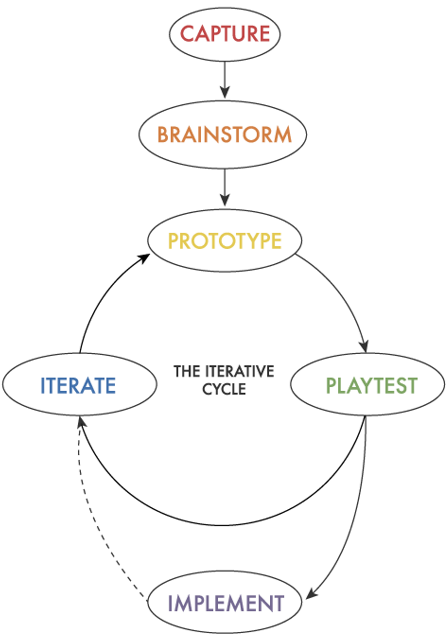
\includegraphics[width=5cm, height=8cm]{Images/IterativeGameDesign.png}}
		\end{figure}
	\section{User Interface}
		The \textbf{design} of the \textbf{User Interface} is meant to \textbf{resemble the original} one in terms of \textbf{screen layout}, but the \textbf{design} and \textbf{some button placements} were changed to suit my \textbf{preferences} and the \textbf{resources available}.

		\subsection{Screen Navigation Architecture}
			The \textbf{player} should be able to have the \textbf{same screen navigation experience} as it would with the \textbf{original game}. 
		\begin{figure}[H]
			\centering
			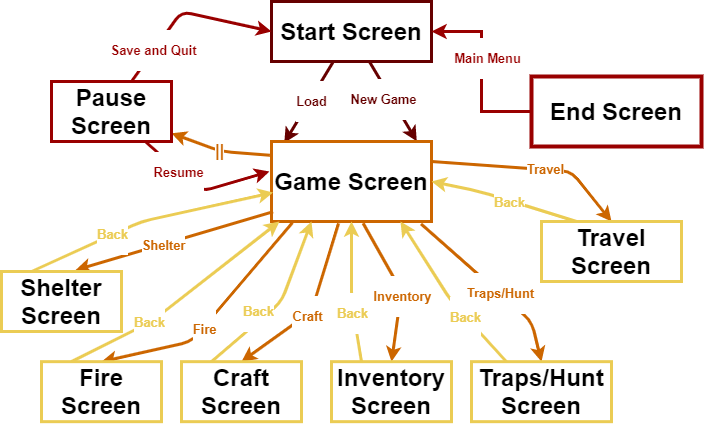
\includegraphics[width=15cm, height=20cm, keepaspectratio]{Images/ScreenArchitecture.png}\\
			\caption{\textbf{Screen Navigation}}
		\end{figure}

		\subsection{Screens}
			\par The entire \textbf{game} can be played with a simple \textbf{screen press}, \textbf{no scrolling} needed(including the inventory). There are \textbf{Pop Up} screens with \textbf{instructions} and \textbf{explanations} when necessary.
			\subsubsection{Main Menu and Pause Screens}
				\begin{figure}[H]
					\centering
					\subfigure[\textbf{Main Menu Screen}]{\label{fig:a}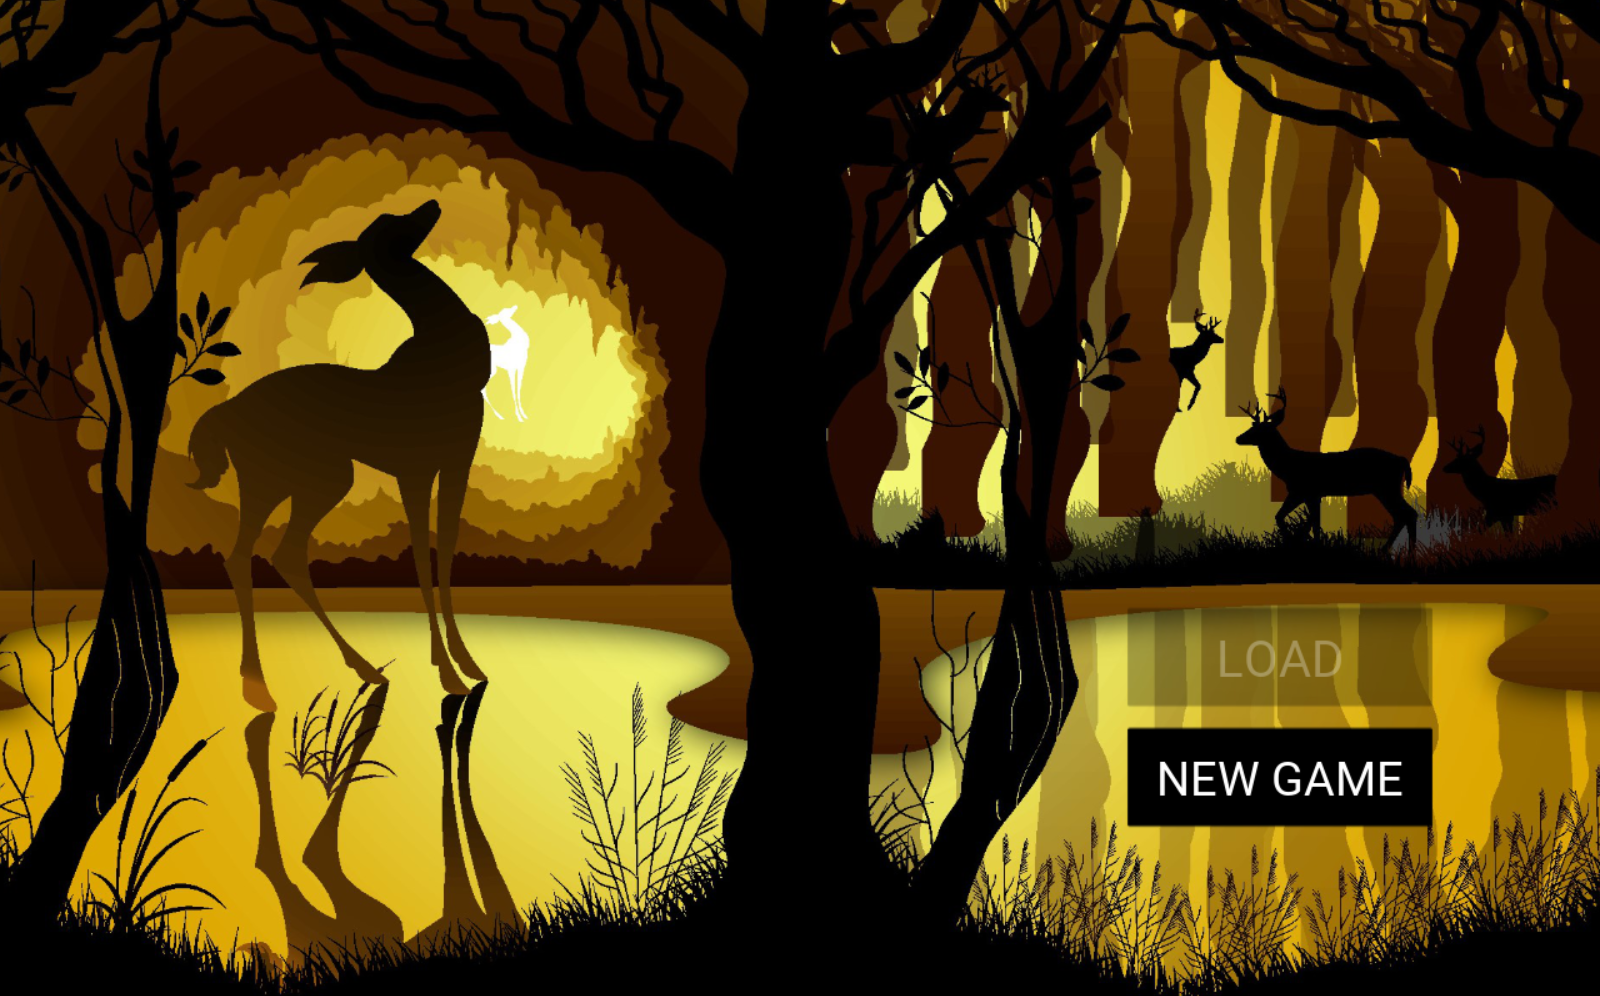
\includegraphics[width=7.5cm, height=4cm]{Images/MainMenu.png}}
				       \subfigure[\textbf{Pause Screen}]{\label{fig:b}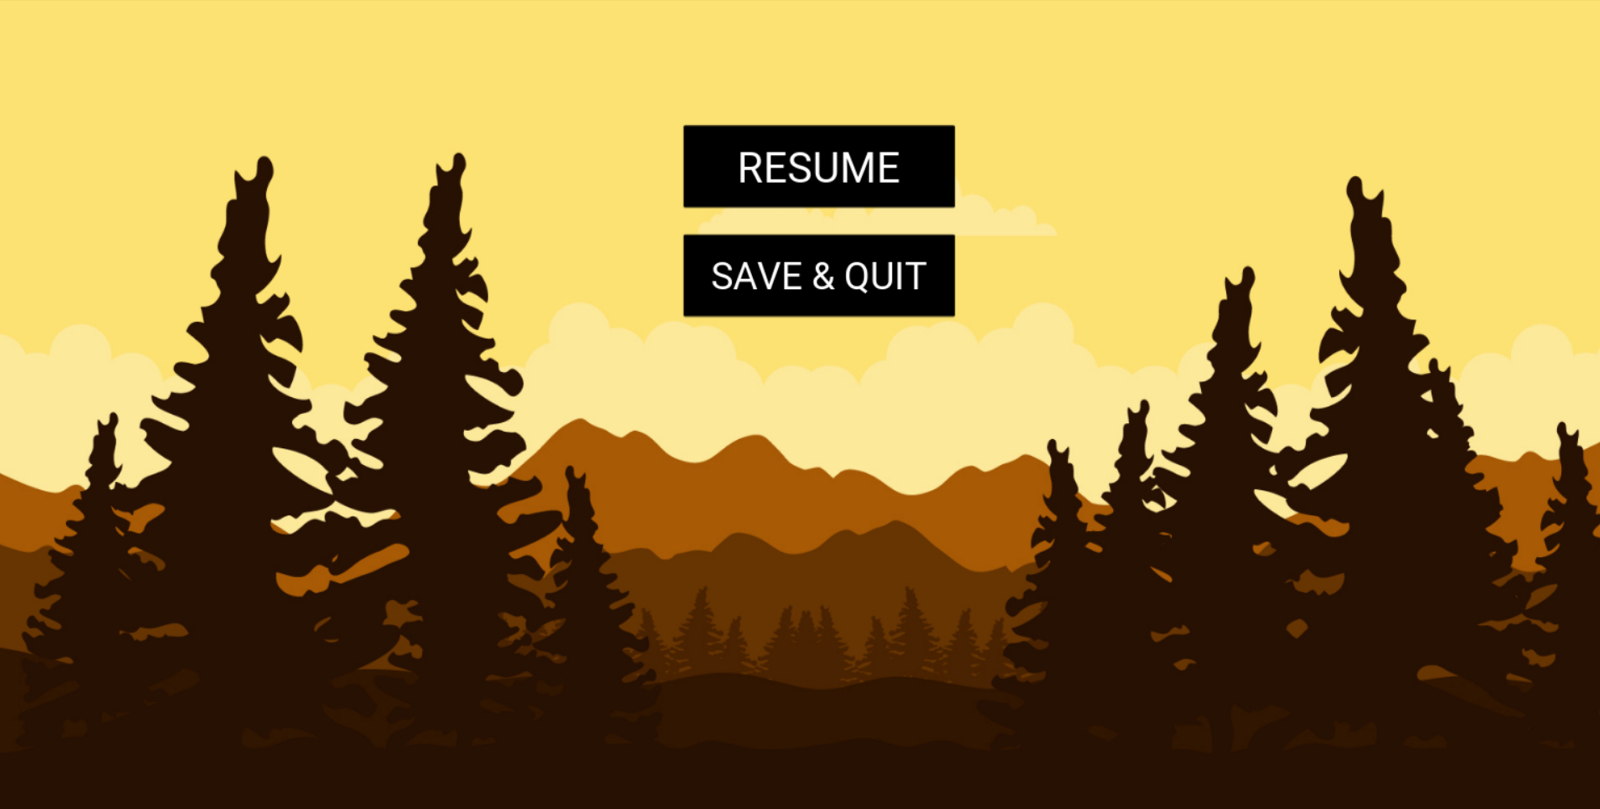
\includegraphics[width=7.5cm, height=4cm]{Images/Pause.png}}
				\end{figure}

			\subsubsection{Game Menu Screen}
				\begin{figure}[H]
					\centering
					\subfigure[\textbf{Game Menu Screen}]{\label{fig:c}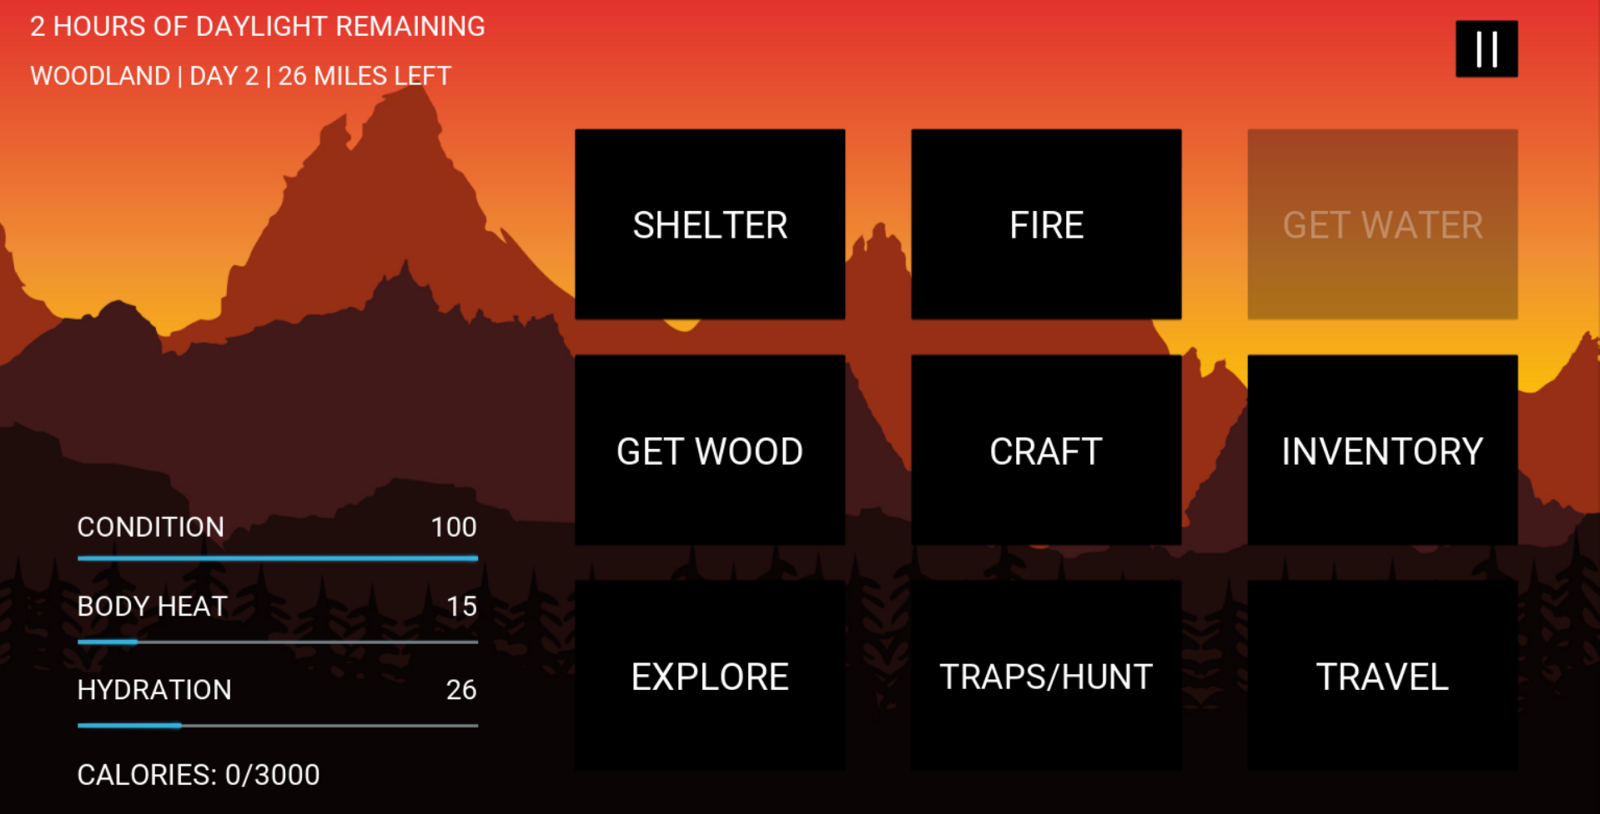
\includegraphics[width=15cm, height=8cm]{Images/Game.png}}
				\end{figure}

			\subsubsection{Crafting Menu Screen}
				\begin{figure}[H]
					\centering
					\subfigure[\textbf{Crafting Menu Screen 1}]{\label{fig:d}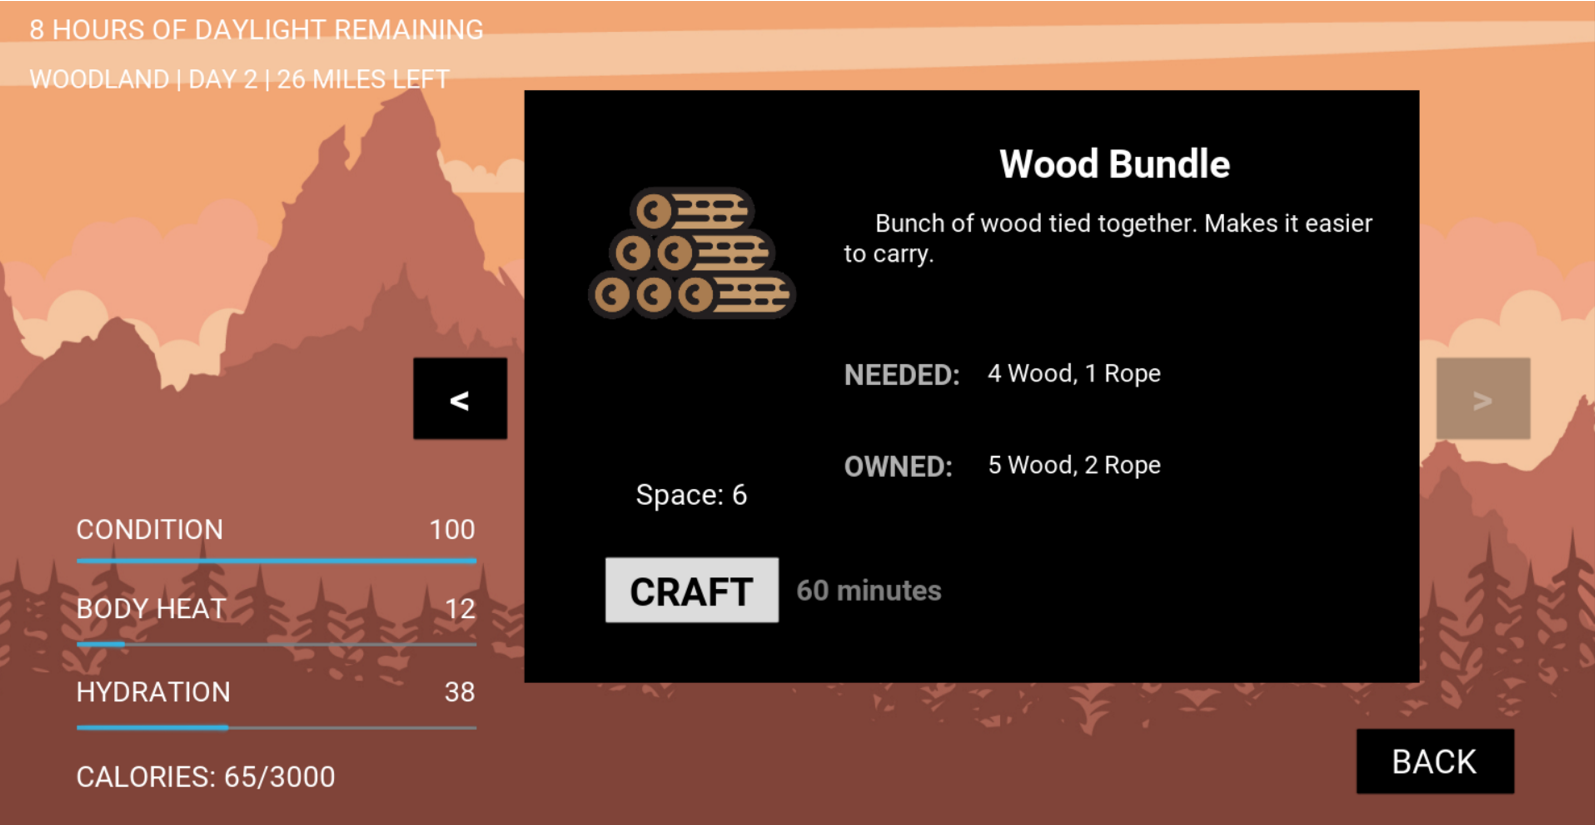
\includegraphics[width=7.5cm, height=4cm]{Images/Craft1.png}}
				       \subfigure[\textbf{Crafting Menu Screen 2}]{\label{fig:e}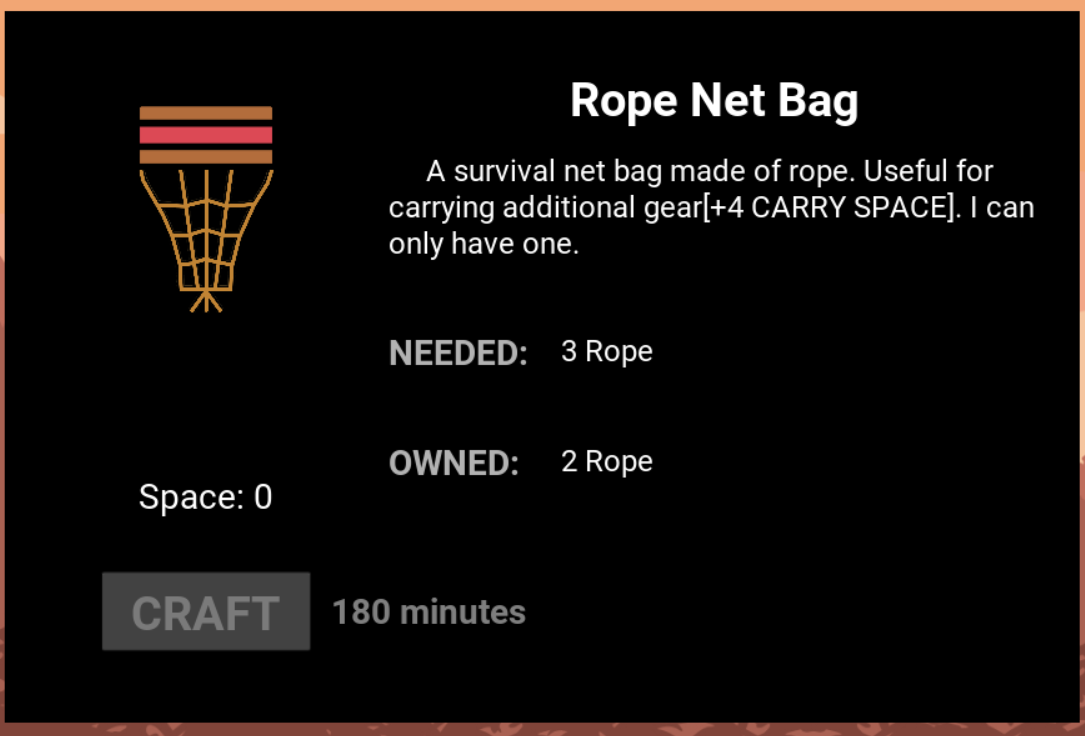
\includegraphics[width=7.5cm, height=4cm]{Images/Craft2.png}}
				\end{figure}

			\subsubsection{Shelter and Traps Screens}
				\begin{figure}[H]
					\centering
					\subfigure[\textbf{Shelter Screen}]{\label{fig:f}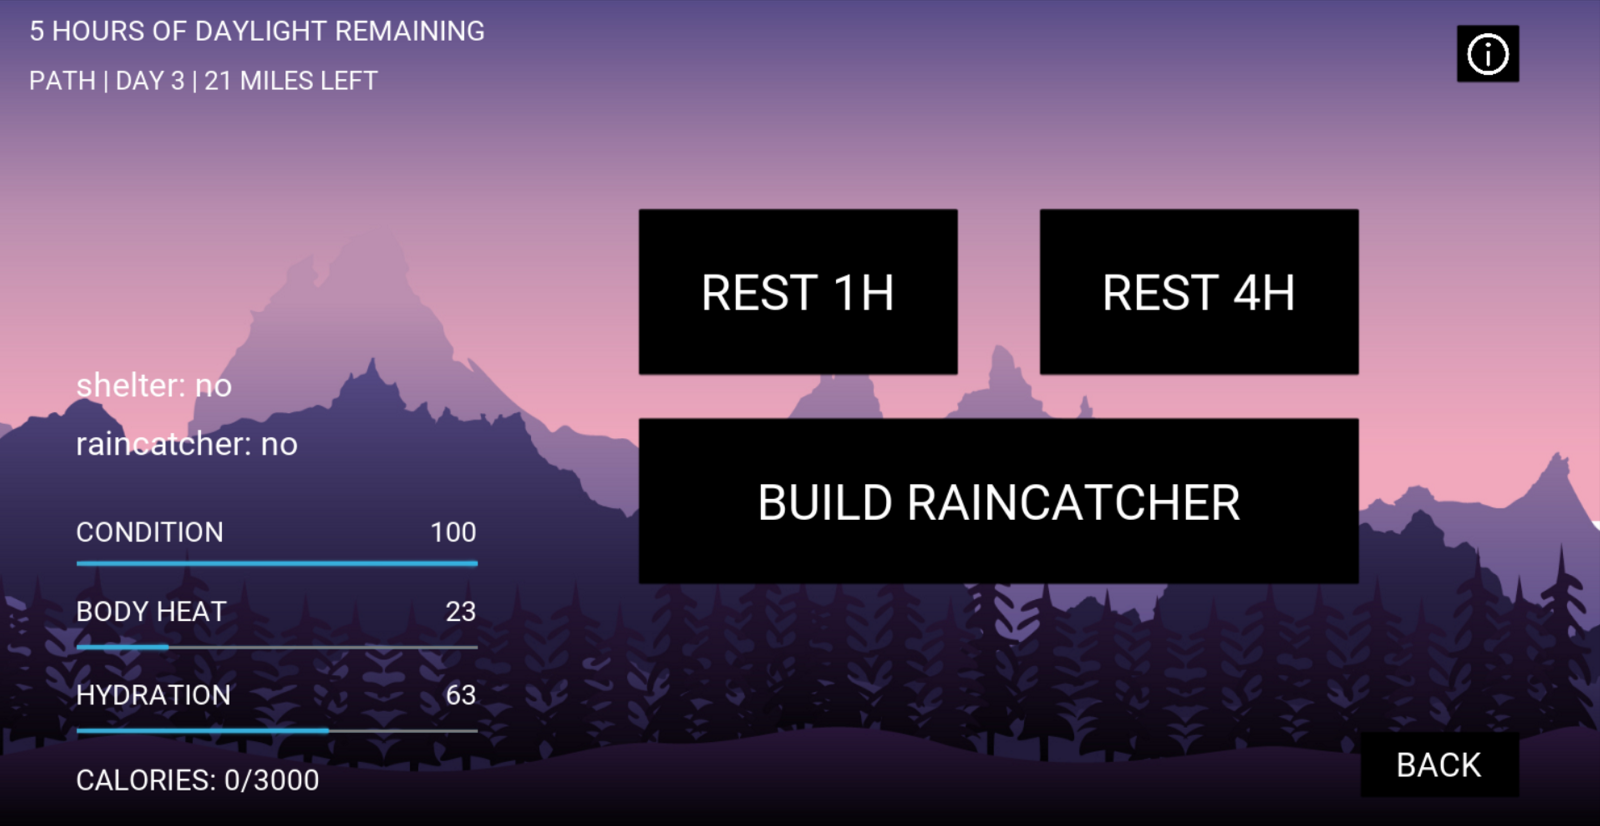
\includegraphics[width=7.5cm, height=3.8cm]{Images/Shelter.png}}
				       \subfigure[\textbf{Traps Screen}]{\label{fig:g}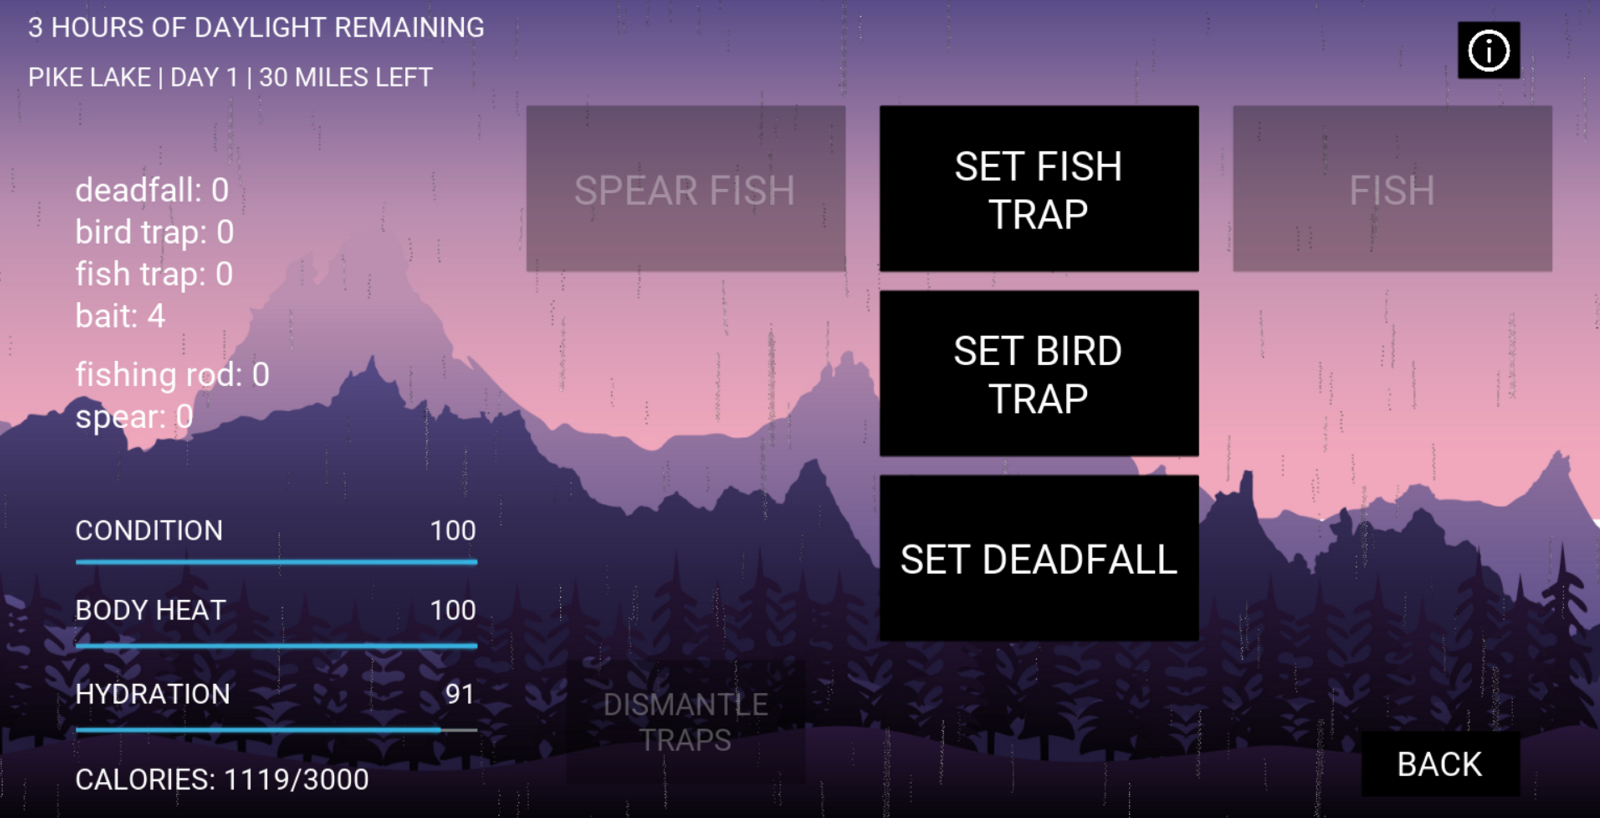
\includegraphics[width=7.5cm, height=3.8cm]{Images/Traps.png}}
				\end{figure}
			\subsubsection{Inventory Screen}
				\begin{figure}[H]
					\centering
					\subfigure[\textbf{Inventory Screen 1}]{\label{fig:j}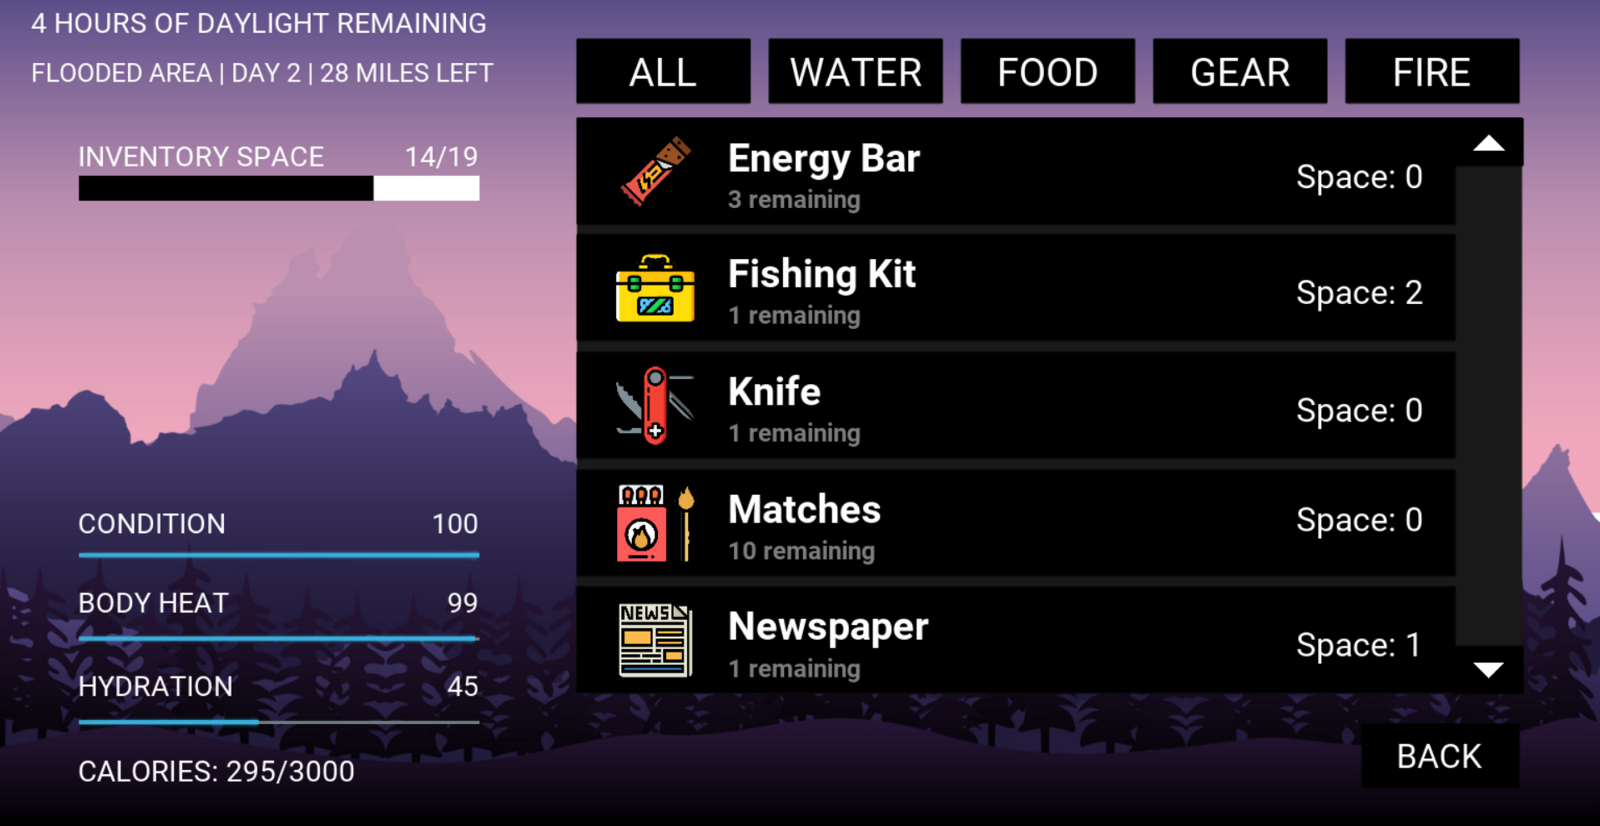
\includegraphics[width=7.5cm, height=3.8cm]{Images/Inventory3.png}}
					\subfigure[\textbf{Inventory Screen 2}]{\label{fig:h}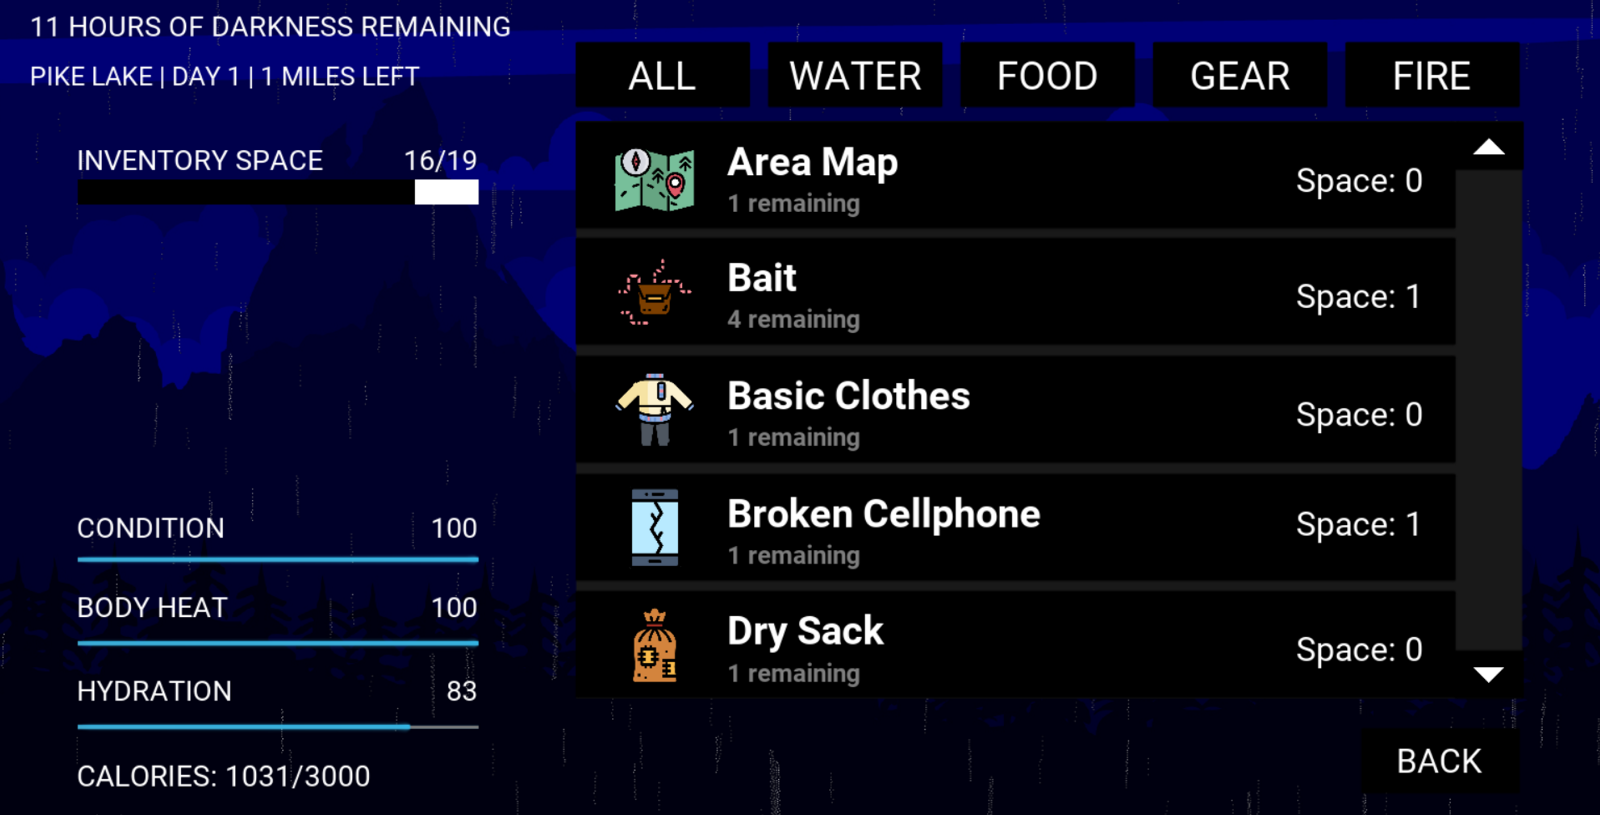
\includegraphics[width=7.5cm, height=3.8cm]{Images/Inventory1.png}}
				\end{figure}
			\subsubsection{Fire Screen}
				\begin{figure}[H]
					\centering
					\subfigure[\textbf{Fire Screen 1}]{\label{fig:l}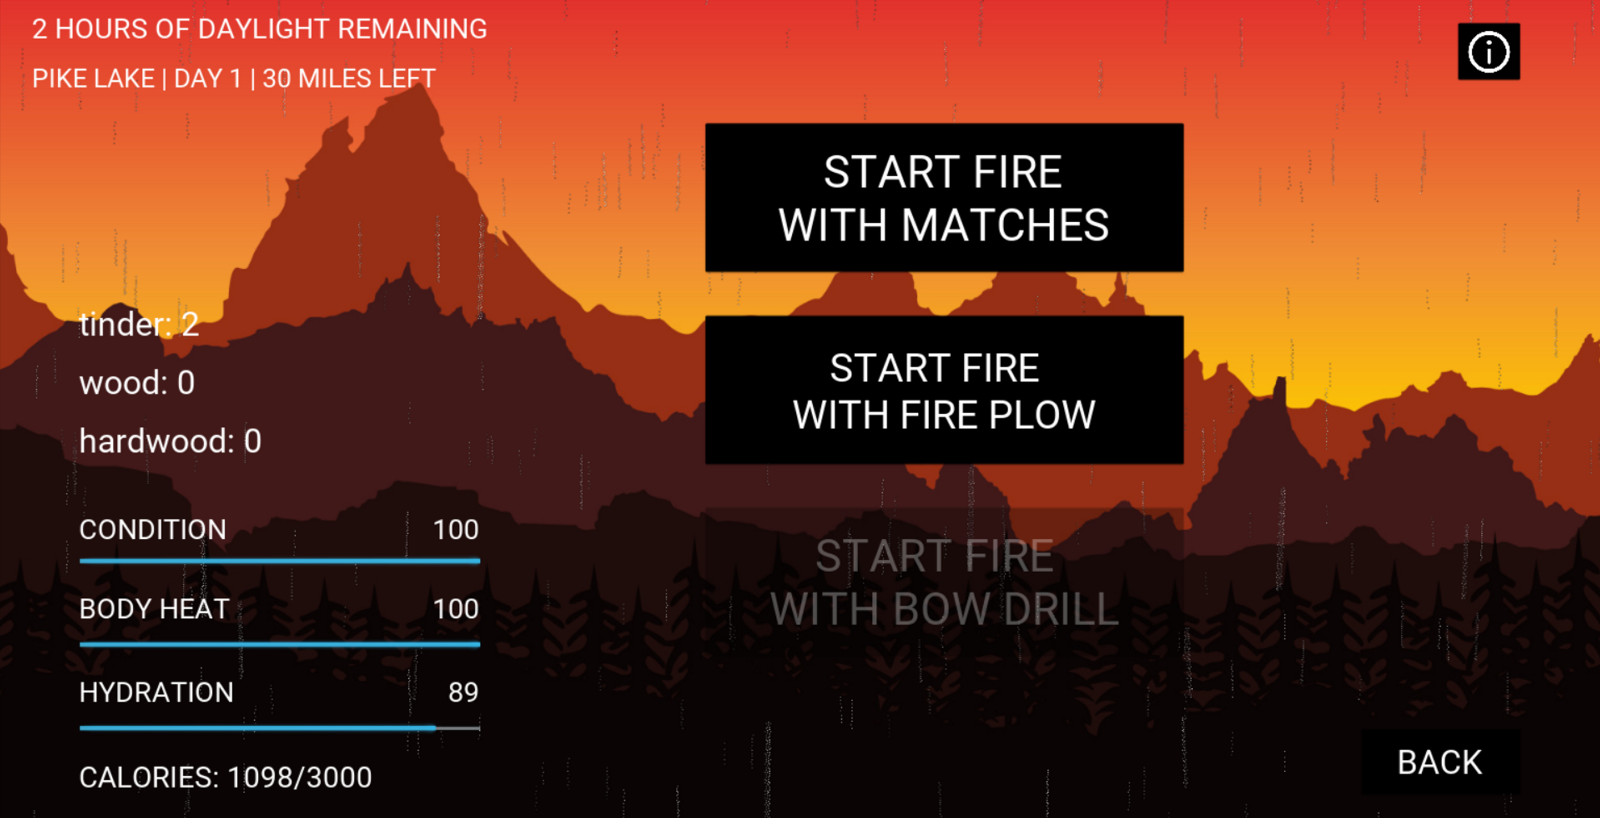
\includegraphics[width=7.5cm, height=3.8cm]{Images/Fire1.png}}
				       \subfigure[\textbf{Fire Screen 2}]{\label{fig:m}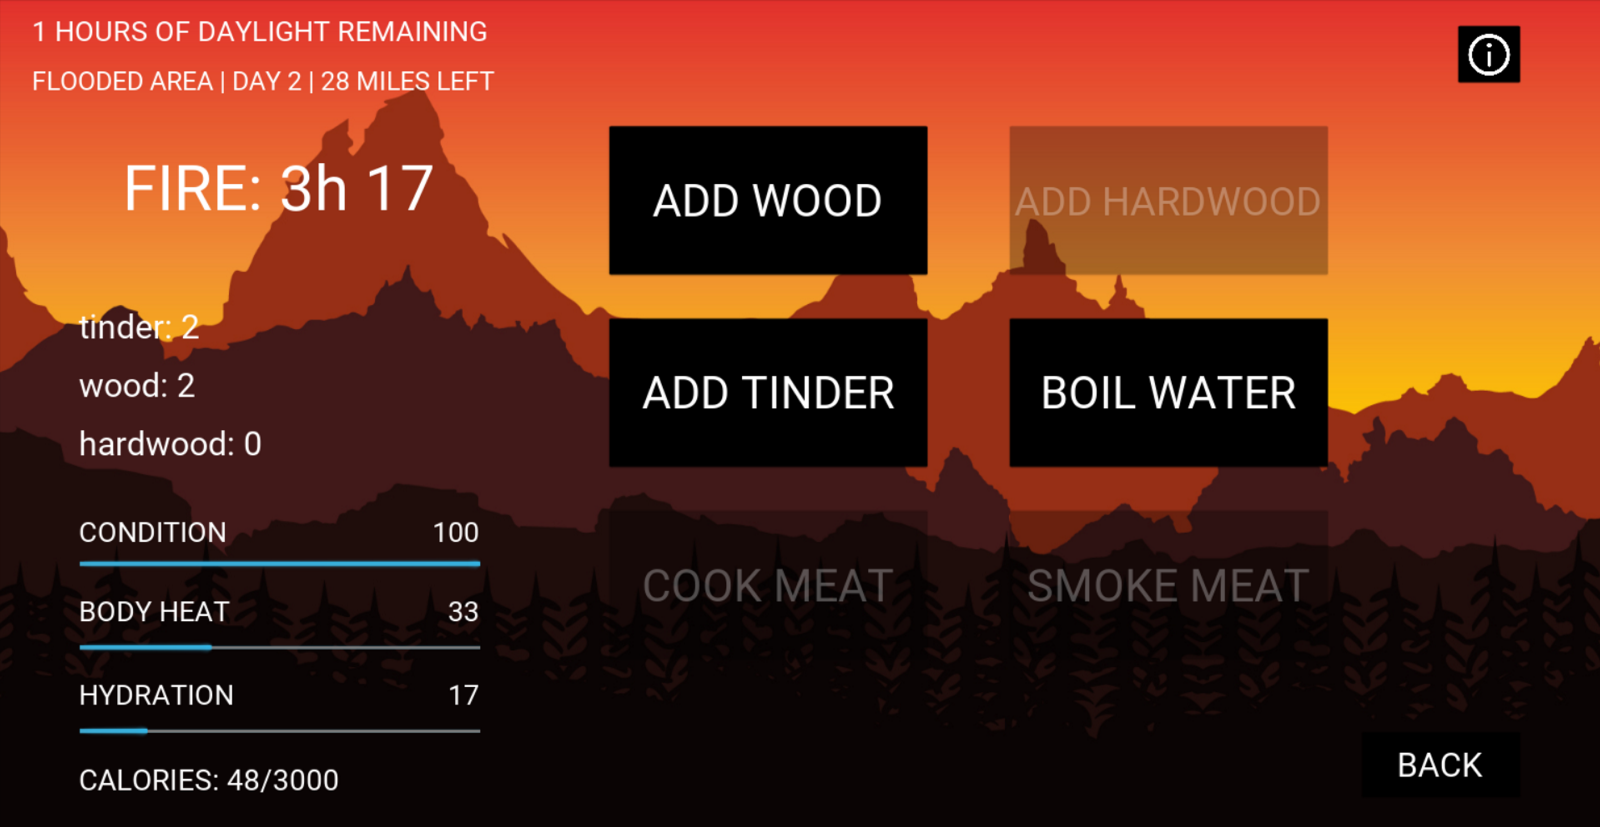
\includegraphics[width=7.5cm, height=3.8cm]{Images/Fire2.png}}
				\end{figure}
			\subsubsection{Travel Screen}
				\begin{figure}[H]
					\centering
					\subfigure[\textbf{Travel Screen}]{\label{fig:n}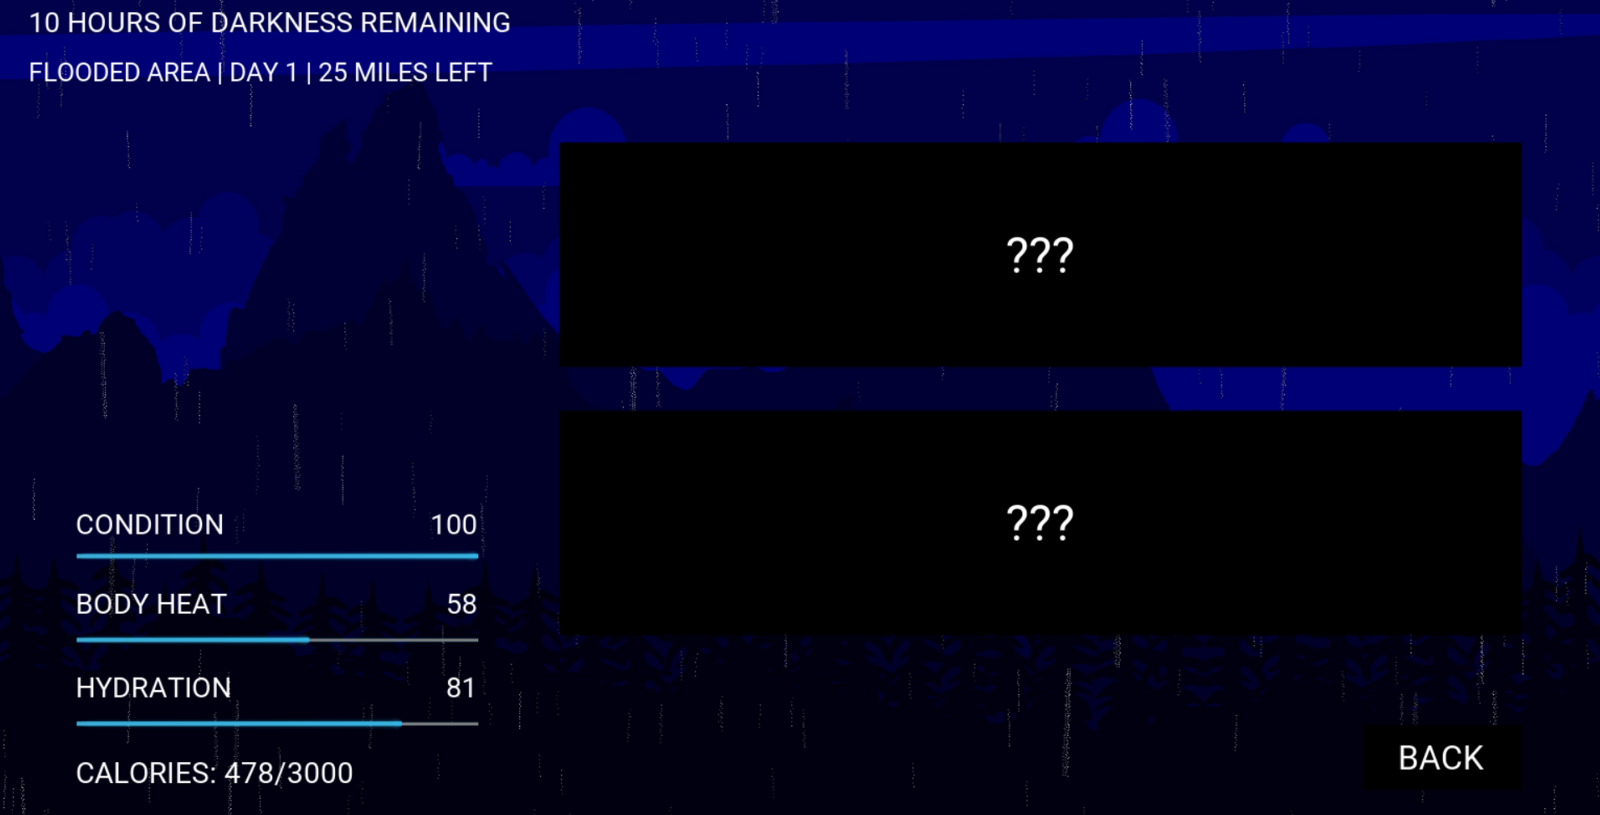
\includegraphics[width=7.5cm, height=3.8cm]{Images/Travel1.png}}
				       \subfigure[\textbf{Travel Screen with Flashlight}]{\label{fig:o}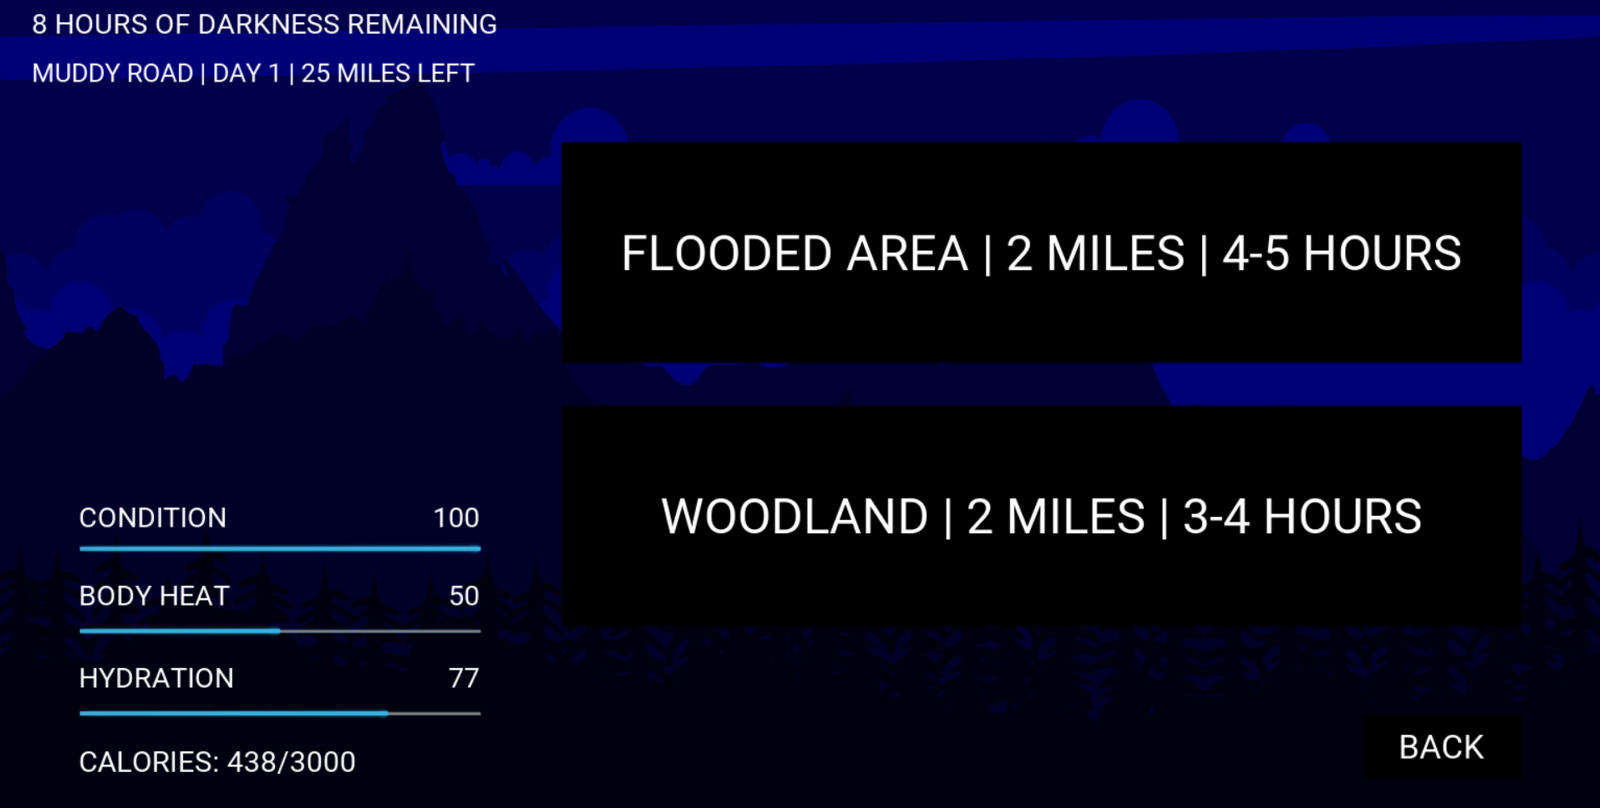
\includegraphics[width=7.5cm, height=3.8cm]{Images/Travel2.png}}
				\end{figure}

			\subsubsection{End Screen}
				\begin{figure}[H]
					\centering
					\subfigure[\textbf{Win Screen}]{\label{fig:p}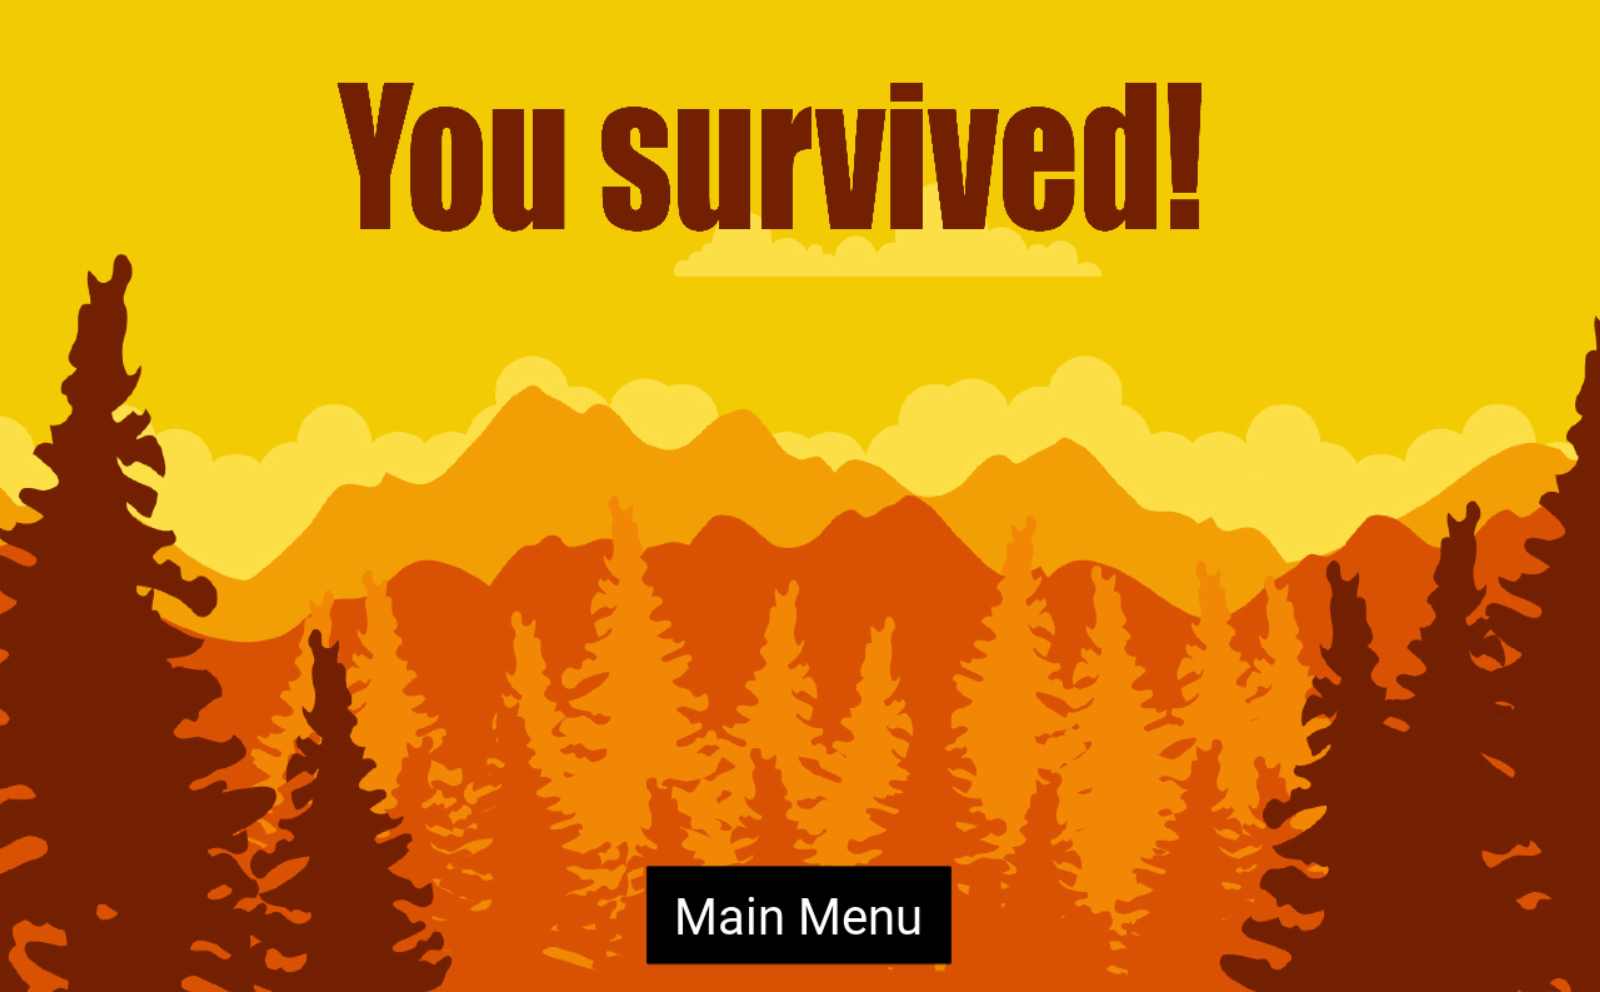
\includegraphics[width=7.5cm, height=4cm]{Images/Win.png}}
				       \subfigure[\textbf{Loss Screen}]{\label{fig:q}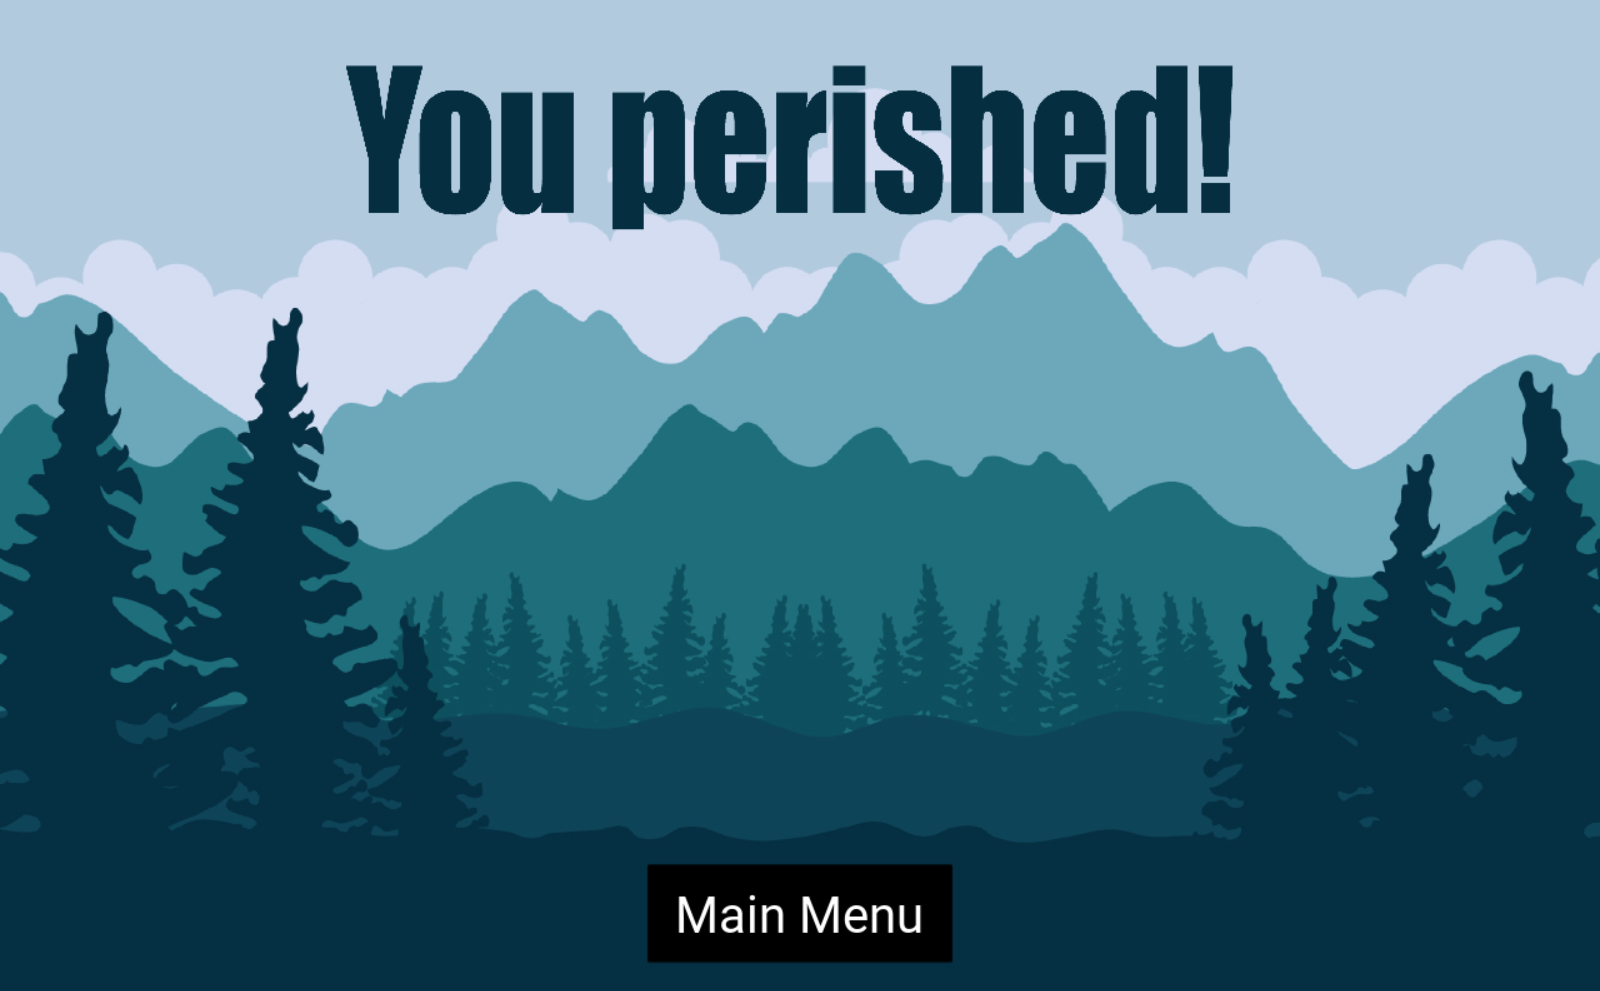
\includegraphics[width=7.5cm, height=4cm]{Images/Loss.png}}
				\end{figure}

\newpage


